\section{Test vehicule description and failure signature}

This chapter focuses on the functionnal failure caused by an \gls{esd} of an integrated function.
The studied function is the primary supply of a complex automotive \gls{asic}.
This supply plays a critical role in the functionning of the entire product.
It is connected to the battery of the vehicle, and is the first block of the product to start.
It wakes up and powers all other functions inside the integrated circuit.

\begin{figure}[h]
  \centering
  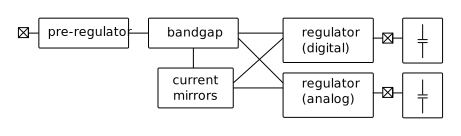
\includegraphics{src/4/figures/testchip_overview.pdf}
  \caption{Architecture of the studied functionnality}
  \label{testchip_overview}
\end{figure}

The primary supply processes the battery supply in a chained fashion (see Fig. \ref{testchip_overview}).
A first block (pre-regulator) clamps the battery voltage (that can reach up to 40V) to 9V, a more acceptable voltage for the silicium technology.
This clamped voltaged is then used to power up a bandgap reference.
Once properly started, this bandgap generates a 1.23 V voltage reference, stable accross a wide range of temperature, process variation and mismatchs.
The bandgap also outputs a 10uA current reference, stable in the same conditions.

After the bandgap, a \gls{ldo} regulator relies on the voltage reference to generate a stable 2.5V supply voltage, able to deliver and sustain up to 20mA.
This first regulator is connected externally to a 100nF decoupling capacitor to absorb peak currents and achieve stability.
This supply is used to supply most analog (digital ?) functions inside the integrated circuit.

A second regulator performs the same task, but starts with a delay compared to the first one.
It also ouputs a 2.5V supply, that powers digital logic inside the circuit.

In case of failure, the primary supply can cause the entire product to shut down.
Indeed, this entire system requires soft-start behavior to avoid generating harmful voltage spikes to powered functions.
This functionnality enforces the system to start on a \br{long} period of time, in the order of a hundred microseconds.

When the system is stressed with an \gls{esd}, voltages and currents are fluctuating inside the block.
Under certain conditions, and especially important stress levels, the block will detects some nodes going in undervoltage or overvoltage.
This will cause the block to go into safe or protected mode, where it will restart because the functionnality cannot be assured properly.
The direct consequence is that the block will require again a hundred microseconds to be again in normal operation mode.

This failure can in a first time be observed in simulation.
An \gls{ESD} is superimposed on the DC battery voltage.
This is the most likely entry point for a stress, because the \gls{IC} exposes a pin to the external workd and is usally connected to the battery via a long cable
To detect is a block reset happened, the voltage on the first voltage regulator is observed.
Fig. X shows the stress waveform on the input.

STRESS WAVEFORM INPUT

Fig. X shows a simulation where a small glitch can be observed on the regulated output, but without clear reset or soft-failure signature.
In this case, the block and the rest of the product is most likely not affected by the ESD.

WAVEFORM OUTPUT NO RESET

Fig. X shows a simulation where a clear reset hapened.
The output voltage is maintained by a 100nF capacitor.
However, it clearly goes down \br{after} the \gls{esd} and rises slowly afterward, a sign that the block went into full reset and restard.

WAVEFORM OUTPUT RESET

By going inside the \gls{IC}...

bandgap, voltage ref, current ref, etc

DISCUSSION AROUND INCREASE OF FAILURE LENGTH after each stage of the chain

\section{Bottom-up block failure modeling}

Consider a system constituted of two blocks A and B connected together.

\begin{figure}[!htbp]
  \centering
  
\includegraphics{src/4/figures/system_ab.pdf}
  \caption{Basic IC function}
  \label{basic_ic_function}
\end{figure}

During normal operation, the \textbf{\textit{out}} signal complies with its specification,
under the condition that the \textbf{\textit{in}} signal does too.
This guarantees that block A and B are performing as expected.

When the system is exposed to an electrical stress on the input during normal operation,
the \textbf{\textit{in}} signal is disturbed.

It no longer complies with its specification, for a given amount of time.

The robustness of the entire system is defined by its ability to maintain signal \textbf{\textit{out}} in specification
while signal \textbf{\textit{in}} is temporarily disturbed.

Time is a key parameter here. On one extreme side, a disturbance that lasts forever is equivalent to the \textbf{\textit{in}} signal not fullfilling its DC specification,
and thus the \textbf{\textit{out}} signal will not fullfill its spec as well.
On the other extreme side, an extremely short disturbance, much shorter than the functionnal timescales of the integrated function will most likely not disturb ??

The first task for defining the robustness of an integrated function is to determine the time threshold under which it can maintain functionnality while being disturbed.
The second key parameter is related to the amplitude of the disturbance, whether it is a voltage, current, energy, etc.
A larger amplitude can make a short pulse more harmful than a lomg one.

\subsection{Block failure characterization and modeling method}
\label{sec:block-failure-cz}

% What is bottom up
In a bottom-up approach, the study focuses first on the small-scale components of a system.
They are characterized individually, and a model is derived for each component.
Afterwards, these models are assembled together to match the full system architecture.
The main idea of a bottom-up approach is that a system is the sum of its parts.
Ultimately, we study if the robustness of a system can be assimilated as the sum of the robustness of its parts.

% Applicability to IC design
This approach fits well with the \gls{asic} design flow in general.
At some point in the design flow, the architecture of the integrated circuit is decided.
Then, each top-level function is split recursively into unit functions to be designed, to simplify the problem.
This part is rather a divide-and-conquer method, where a complex problem is split up into multiple simpler tasks.

Then, the design phase starts. It is a bottom-up method.
Transistors are assembled together to perform (usually one) unit function into what is called a \gls{block}.
Those blocks are then assembled together to build the more complex and interesting functionnalities.

% Why bottom up
The main perk of this characterization method is the inherent modularity.
The objective is to study each block independently of the others.
This way, the model built for each block is reusable.
A characterized block can be reused multiple times without having to do the characterization again each time.

% How is it done, core concept
The method described in this section starts by characterizing each block in a particular setup.
This setup provides appropriate biasing to the block, in order to set it in normal operating conditions.
This setup is also in charge of injecting the characterization signal on the tested input, and monitoring of the output under test.
Fig. \ref{block_function_cz} gives an example of such a characterization setup for a supply input.

\begin{figure}[!htbp]
  \centering
  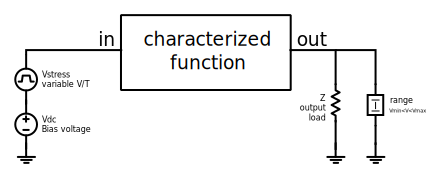
\includegraphics{src/4/figures/characterization_setup.pdf}
  \caption{Block characterization setup (supply input)}
  \label{block_function_cz}
\end{figure}

% What are the characterization signal
The characterization signal is a square waveform, applied on the tested input.
A set of simulations is ran with this setup.
Each simulation runs with a different pair of values for the \textbf{amplitude} and \textbf{duration} of the square signal.
Table \ref{parameterized-simulations} illustrates this simulation process.
Such testing method is called Wunsch and Bell in the litterature (REFERENCE).

\begin{table}[!htbp]
\centering
\begin{tabular}{@{}lllll@{}}
\toprule
    & 1ns   & 10ns  & 100ns & 1us   \\ \midrule
5V  & sim11 & sim21 & sim31 & sim41 \\
10V & sim12 & sim22 & sim32 & sim42 \\
15V & sim13 & sim23 & sim33 & sim43 \\ \bottomrule
\end{tabular}
\caption{Parameterized simulation planning for the characterization}
\label{parameterized-simulations}
\end{table}

In the time domain, this set of simulations is illustrated in Fig. \ref{set_input_signals}.

%TODO: Fix sim 12 sim12
\begin{figure}[!htbp]
  \centering
  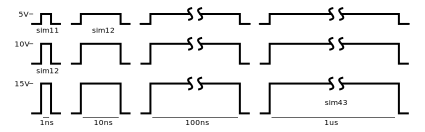
\includegraphics{src/4/figures/time_domain_cz_curves.pdf}
  \caption{Variations on (amplitude, duration) of the input characterization signal}
  \label{set_input_signals}
\end{figure}

% What is the direct result of the characterization, how to obtain it
For each simulation, the waveform of the output under test is recorded.
The waveform is compared against a threshold.
This threshold can also be seen as failure criteria of the studied function.

This treshold is set prior to the simulation.
There is no general rule for setting it.
The \gls{dc} specification of the output can be used directly, if it exists, or a sound value in regard of the design, or an arbitrary level.

If the waveform goes above (maximum threshold) or below (minimum threshold), the simulation is marked as \textit{fail}.
For each simulation, the duration during which the failure criteria was violated is also recorded.
Once all simulations are complete, it is known which ones contain a \textit{fail}.

The results are summarized into table \ref{simulation-results}.

\begin{table}[!htbp]
\centering
\begin{tabular}{@{}lllll@{}}
\toprule
    & 1ns                          & 10ns                         & 100ns                        & 1us                          \\ \midrule
5V  & {\color[HTML]{32CB00} sim11} & {\color[HTML]{32CB00} sim21} & {\color[HTML]{32CB00} sim31} & {\color[HTML]{FE0000} sim41} \\
10V & {\color[HTML]{32CB00} sim12} & {\color[HTML]{FE0000} sim22} & {\color[HTML]{FE0000} sim32} & {\color[HTML]{FE0000} sim42} \\
15V & {\color[HTML]{FE0000} sim13} & {\color[HTML]{FE0000} sim23} & {\color[HTML]{FE0000} sim33} & {\color[HTML]{FE0000} sim43} \\ \bottomrule
\end{tabular}
\caption{Example of results on a set of simulations (simulations in red contain a fail)}
\label{simulation-results}
\end{table}

% A first visualization of the characterization
A curve can be build from this table, to make visualization easier.
It gives a visual representation of the functionnal robustness of the block.
Following table \ref{simulation-results}, the x axis is the duration of the input stress.
The y axis is the amplitude of the input signal during the stress.
This amplitude is the voltage or current seen by the characterized input pin.
It is the sum of the stress amplitude and an eventual biasing level.
Finally, each point (x,y) of the curve represents the \textbf{minimal} amplitude (y) for the given pulse width (x) at which failures occur.

Fig. \ref{wb_cz_curve_example} gives an example of such a characterization curve.

%TODO: REVOIR COULEURS
\begin{figure}[!htbp]
  \centering
  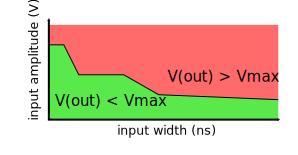
\includegraphics{src/4/figures/example_curve.pdf}
  \caption{Principle of Wunsch and Bell curve for powered-on block testing}
  \label{wb_cz_curve_example}
\end{figure}

% How to improve the displayed information
The duration during which an output is in fail was recorded for each simulation, as stated earlier.
% WHY IS THIS IMPORTANT
It is possible to improve table \ref{simulation-results} by replacing the \textit{fail} by the duration of the fail.
This is illustrated in table \ref{simulation-results-bis}.

\begin{table}[!htbp]
\centering
\begin{tabular}{@{}lcccc@{}}
\toprule
    & \multicolumn{1}{l}{1ns}      & \multicolumn{1}{l}{10ns}     & \multicolumn{1}{l}{100ns}    & \multicolumn{1}{l}{1us}     \\ \midrule
5V  & {\color[HTML]{32CB00} }      & {\color[HTML]{32CB00} }      & {\color[HTML]{32CB00} }      & {\color[HTML]{F56B00} 2us}  \\
10V & {\color[HTML]{32CB00} }      & {\color[HTML]{00D2CB} 125ns} & {\color[HTML]{F8A102} 540ns} & {\color[HTML]{FE0000} 30us} \\
15V & {\color[HTML]{00D2CB} 110ns} & {\color[HTML]{FFCB2F} 150ns} & {\color[HTML]{FE0000} 30us}  & {\color[HTML]{FE0000} 30us} \\ \bottomrule
\end{tabular}
\caption{A more informative representation of all simulation results to account for duration of output failure}
\label{simulation-results-bis}
\end{table}

% How to improve the curve from the improved table
This improvement can also be transfered to the curve representation.
A gradient can be used rather than a simple failure curve.
For each point of the curve, the gradient will have a value representing the duration of the failure on \textbf{\textit{V(out)}}.
The figure \ref{wb_cz_curve_example_v2} provides an example of this improved representation.
In this figure, the warmer the gradient, the longer the output is disturbed.

\begin{figure}[!htbp]
  \centering
  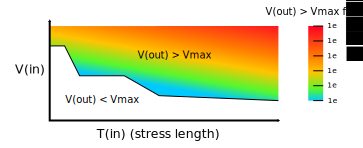
\includegraphics{src/4/figures/example_curve_v2.pdf}
  \caption{Improved curve for Wunsch and Bell powered-on characterization}
  \label{wb_cz_curve_example_v2}
\end{figure}

The gradient can also be discretized into a few aeras for better readability as shown in figure \ref{wb_cz_curve_example_v2_discrete}.
This representation looses some information compared to the gradient one, but is easier to generate and read.
This is the representation we have adopted further in this study, to express the functionnal robustness of a single block.

\begin{figure}[!htbp]
  \centering
  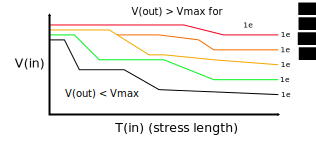
\includegraphics{src/4/figures/example_curve_v2_discrete.pdf}
  \caption{Improved discrete curve for Wunsch and Bell powered-on characterization}
  \label{wb_cz_curve_example_v2_discrete}
\end{figure}

\subsection{Block models chaining}
\label{sec:block-chaining}

% Explain the chaining mechanism
The characterization process detailed previously (in \ref{sec:block-failure-cz}) is repeated on each block constituting a high-level function.
Once done, the bottom-up study now focuses on a higher level in the design hierarchy.
As a remainder, the original goal of this method is to see if the robustness of a high-level function is the sum of its parts' robustness.

Thus, individual models are connected together, by following exactly how blocks are connected in the design.
To illustrate this idea, fig. \ref{example_toplevel_function} represents an example of a high-level function, constituted of three blocks at the second level of hierarchy.
It is assumed that each of these blocks has been characterized.

% WHICH NET IS TOP MONITORED ?

\begin{figure}[!htbp]
  \centering
  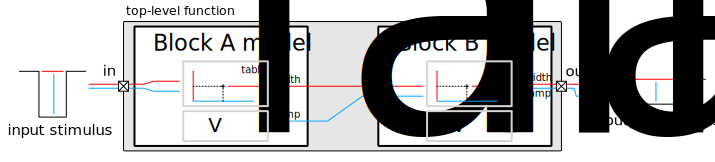
\includegraphics{src/4/figures/example_top_level_function.pdf}
  \caption{Example of a top-level function with 3 characterized blocks}
  \label{example_toplevel_function}
\end{figure}

% Remind the final goal
Now, we want to obtain the robustness of the entire function, against a given stress, using the block models.
The stress is injected on the global pin \textbf{\textit{in}}.

% What is the input stress ? What is the top-level function evaluated against ?
In this example, we will consider the stress is generated by a \gls{tlp} generator, and is thus rectangular.
For this example, the stress is chosen to have a duration of 100 ns, and an amplitude of 10V.
Section \ref{sec:wb-for-arbitrary-wvfs} describes methods for applying the block models to arbitrary input waveforms.

The stress is injected on the global \textbf{\textit{in}} pin.
This pin is also the input pin of the first block.
Thus, the properties of the \gls{tlp} pulse can directly be applied to the model of block A.
Fig. \ref{example_complete_curve} shows an example curve for model A, and the location of the TLP pulse characteristics on this curve.


\begin{figure}[!htbp]
  \centering
  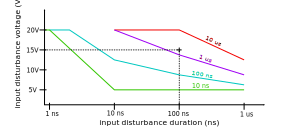
\includegraphics{src/4/figures/example_complete_curve.pdf}
  \caption{Model A curve and determination of impact of the TLP pulse - values in color represent the duration of failure on the output}
  \label{example_complete_curve}
\end{figure}

% Interpretate stress to deduce net1
Like stated earlier, the pulse has a duration of 100ns and an amplitude of 15V. By reporting this point on curve \ref{example_complete_curve},
it is visible that this will cause the output of block A to violate its failure criteria between 1us and 10 us.
We consider, for the sake of this example, the failure criteria of block A to be net1 > 5V.
With a 100ns long 15V pulse on the input of A, the characterization states that the output of block A will go above 5V for at least 1us.
This is the best case value for net1.

% Use net1 as input of next block
\textit{net1} is the output of block A, but it is also the input of block B.
Thus, best case (amplitude, duration) values for net1 can be used as input for block B's model.
Fig. \ref{example_complete_curve_B} shows an example curve for model B, and the location of the \textit{net1} disturbance on this curve.
This shows that \textit{net2}, the output of block B and the input of block C, will go below B's failure level for at least 10 us.

\begin{figure}[!htbp]
  \centering
  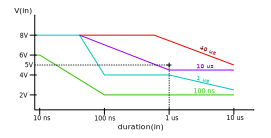
\includegraphics{src/4/figures/example_complete_curve_B.pdf}
  \caption{Model B curve and determination of impact of the TLP pulse}
  \label{example_complete_curve_B}
\end{figure}

% Repeatable process
As shown, this process can be repeated in theory with as many blocks as required by the original design, until the final pin is reached.
The is possible because the output of a block is used as the input of the next one.

% How to select pins to characterize

% Show how it can help to speedup and simplify the computation of the entire function robustness

\subsection{Application to the test vehicle}

The method described in both previous sections (\ref{sec:block-failure-cz} and \ref{sec:block-chaining}) is tested in simulation on real blocks.
More precisely, it will be tested against the regulation function of the testchip.

% Which pins are selected for characterization
This function is composed of three blocks, a pre-regulator, a bandgap and a regulator.
For each one, an input and output pin are selected.
The input/outputs that play a key role on the regulation function were selected on the regulation function.
Details of the selected pins is given in Table \ref{selected-pins-for-cz}.

% TODO : Give more pins and just indicates the one that were chosen ?
\begin{table}[!htbp]
\centering
\resizebox{\textwidth}{!}{%
\begin{tabular}{@{}|c|c|c|c|c|@{}}
\toprule
{\color[HTML]{000000} \textbf{IC block}} & \multicolumn{2}{c|}{{\color[HTML]{000000} \textbf{input}}}                                                                                                                                                 & \multicolumn{2}{c|}{{\color[HTML]{000000} \textbf{output}}}                                                                                        \\ \midrule
{\color[HTML]{000000} }                  & {\color[HTML]{000000} \textbf{function}}                                                            & {\color[HTML]{000000} \textbf{\begin{tabular}[c]{@{}c@{}}characterization\\ range (V)\end{tabular}}} & {\color[HTML]{000000} \textbf{function}}                                                        & {\color[HTML]{000000} \textbf{Failure criteria}} \\ \midrule
{\color[HTML]{000000} pre-regulator}     & {\color[HTML]{000000} \begin{tabular}[c]{@{}c@{}}external supply\\ battery connection\end{tabular}} & {\color[HTML]{000000} {[}0V ; -10V{]} ?}                                                             & {\color[HTML]{000000} \begin{tabular}[c]{@{}c@{}}9V clamped\\ voltage\end{tabular}}             & {\color[HTML]{000000} V \textless 5V ?}          \\ \midrule
{\color[HTML]{000000} bandgap}           & {\color[HTML]{000000} \begin{tabular}[c]{@{}c@{}}9V clamped\\ voltage\end{tabular}}                 & {\color[HTML]{000000} {[}0V ; -5V{]} ?}                                                              & {\color[HTML]{000000} \begin{tabular}[c]{@{}c@{}}bandgap voltage\\ 1.25V ?\end{tabular}}        & {\color[HTML]{000000} V \textless 1.3V ?}        \\ \midrule
{\color[HTML]{000000} regulator}         & {\color[HTML]{000000} bandgap 1.25 V}                                                               & {\color[HTML]{000000} {[}0V ; -3V{]} ?}                                                              & {\color[HTML]{000000} \begin{tabular}[c]{@{}c@{}}regulated 2.5V\\ 20mA capability\end{tabular}} & {\color[HTML]{000000} V \textless 2.2 V?}        \\ \bottomrule
\end{tabular}%
}
\caption{Selected pins for characterization and characterization limits}
\label{selected-pins-for-cz}
\end{table}

% Talk about the characterization limits and failure criteria chosen
%TODO: Detail how were chosen failure criteria
The characterization is done using negative voltages.
The goal is to exploit the weakness of the testchip against negative pulses discovered and highlighted in section \ref{sec:testchip_study}.
Basically, it was observed for sufficiently high negative voltage that a short pulse can cause a full restart of the system.
The time taken by this restart, observed on the regulator output, is several order of magnitudes longer than the original pulse injected on the pre-regulator input.
The failure criteria for the pre-regulator corresponds to XXX ?
The failure criteria for the bandgap output voltage is the DC specification ?
Finally, the failure criteria for the regulator, and thus for the complete function, corresponds to the DC specification of this function.

% Which load value for characterization
The test setup described in section \ref{sec:block-failure-cz} requires a characterization load to simulate the impact of neighbor blocks.
In a first time, a very simplistic model is employed for this load.
An arbitrary load value of 1M\textgreek{Omega}\ is initially chosen, just to perform a preliminary test.
%TODO: DETAIL MORE ?

% Simulation process
For each block, the characterization testbench is setup and a set of simulations is run.
This set is calculated with the characterization range given in Table \ref{selected-pins-for-cz}.
This type of parameterized simulations can be efficiently distributed on multiple machines.
This way, the complete characterization of a block does not take longer than the time taken by a single simulation.
Once all simulations are run, the results are analysed and plotted using the method detailed in the previous sections.

% Talk about the output
These characterization curves are given in Figs. \ref{pre_regu_wb}, \ref{bandgap_wb} and XXX.
For the given testchip, it was found that the regulation function shows clear failure when exposed to negative stresses.
For simplicity, the voltage scale was simply reversed, but this doesn't affect the results in any case.

%TODO: REVERT Y SCALE ON ALL CURVES

\begin{figure}[!htbp]
  \centering
  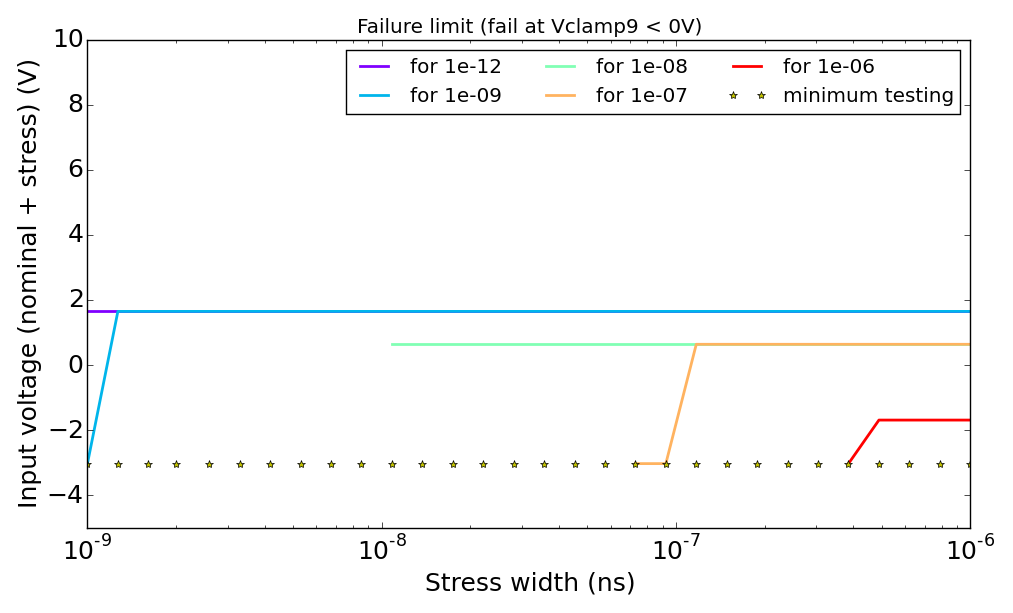
\includegraphics[width=\textwidth]{src/4/figures/cz_vpre.png}
  \caption{Testchip's pre-regulator Wunsch and Bell characterization}
  \label{pre_regu_wb}
\end{figure}

\begin{figure}[!htbp]
  \centering
  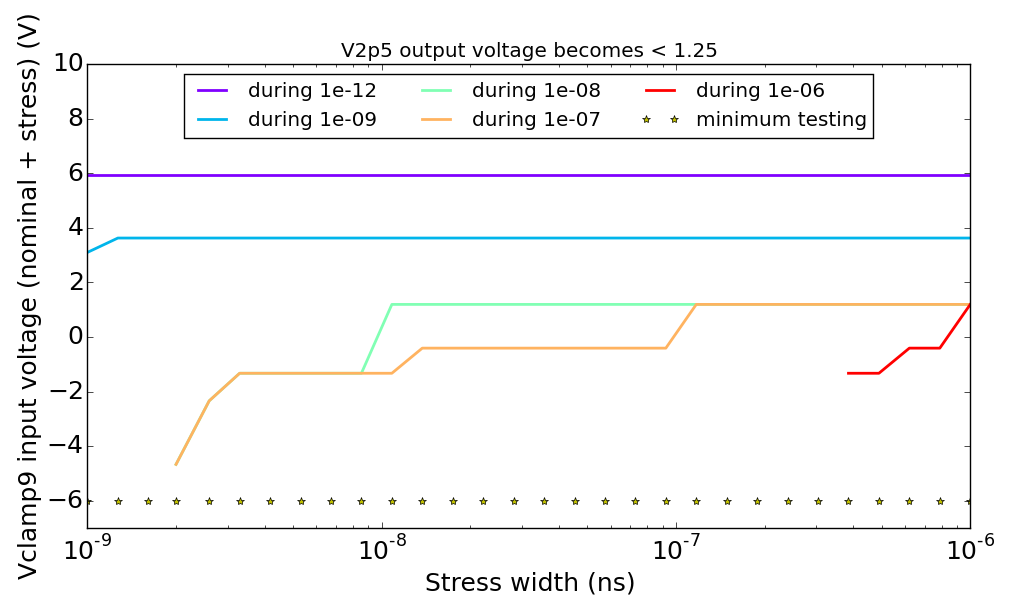
\includegraphics[width=\textwidth]{src/4/figures/cz_bandgap.png}
  \caption{Testchip's bandgap Wunsch and Bell characterization}
  \label{bandgap_wb}
\end{figure}

%TODO: CURVE CZ REGULATOR

% Characterization done, now perform chaining
After the characterization phase, it is now possible to chain the models together to evaluate the entire function's robustness, using method described in \label{sec:block-chaining}.
To check the validity of the model, a rectangular pulse is injected on the global input (pre-regulator input).
The chain of models is used to predict, without running any more simulations, the failure or not on the output pin.
For the purpose of this test, the input stress will be generated by a \gls{tlp} generator, producing a pulse of 100ns duration and -50V amplitude.

% Do it on one pulse config
First, the coordinaates (100ns, -50V) are reported on curve \ref{pre_regu_wb}, the first block model of the system.
This point indicates a failure on the output of the pre-regulator, for a duration between XXns and XXns.
This gives the next point coordinates (XXns, -XXV).
This point is reported on the bandgap's model, the next block in the system.
Using these coordinates in the curve \ref{bandgap_wb} indicates a failure on the bandgap output between XXns and XXXns.
Finally, the point corresponding to the best-case output of the bandgap (XXXns, -XXV) is used as an input for the final block.
This gives a failure on the final output comprised between XXXns and XXXX ns.
In conclusion, the model chain estimated that for a -50V 100ns stress on the input, the regulation function will be at fault (output < XXV) for more than XXXX ns.

%TODO: SHOW ALL THREE CZ CURVES WITH POINT REPORT FROM ONE TO ANOTHER

% Perform standard complete simulation for reference
This result is then tested against a complete simulation of the entire regulation function (all three block).
The simulation circuit is given Fig. X.
This simulation uses transistor-level models, and will serve as a reference to compare the model-chain against it.
The same (100ns, -50V) rectangular pulse will be injected on the global input, and the global output will be monitored as well.
To check the validity of the model, we also monitor intermediate voltages, at the output of the pre-regulator and the bandgap.
The simulation of the input, pre-regulator output, bandgap output and final (regulator) output are given fig. X.

%TODO: SCHEMATIC FULL CIRCUIT

%TODO: PLOT TRANSIENT SIMULATIONS, USING 2 * 2 GRID, PLOTTING INPUT, PRE_REG_OUT, BANDGAP_OUT and REGU_OUT

% Result of the simulation
The simulation showed that for the given stress, the output will go below XXV for XXXns.
There is a rather large difference with the model chain.
To try to explain this difference, intermediates nodes are monitored.

% Error at the first block
The output of the pre-regulator is below X V (failure criteria) for XX ns in the full simulation while the model predicted XX ns.
Already, at this first block, there is a large difference between the simulation and the model.

% Error at the second block
The output of the bandgap (second block) shows even a higher difference.
In simulation, the output goes below XX V for XXX ns, while the model predicted XXX ns.

% Conclusion regarding this first simulation
Not only each curve introduces an important error, but errors tend to accumulate after each block.

% Test further simulation vs model
To test further the model versus the reference simulation, a set of different stresses are injected, with different properties.
The goal is to test the model on a larger set of input stresses.
For each stress, the result predicted by the model and the result obtained by the reference simulation are compared.
Results are summarized in table \ref{tab:comparison-multiple-pulses}.
The entire process is summarized in fig. X.

\begin{table}[!htbp]
\centering
\begin{tabular}{@{}|c|c|c|c|@{}}
\toprule
\multicolumn{2}{|c|}{\begin{tabular}[c]{@{}c@{}}Stress\\ properties\end{tabular}} & \multicolumn{2}{c|}{Results} \\ \midrule
duration (ns)                           & amplitude (V)                           & Reference      & Model       \\ \midrule
1 ns                                    & -5V                                     & no fail        & no fail     \\ \midrule
1 ns                                    & -10V                                    &                &             \\ \midrule
1 ns                                    & -15V                                    &                &             \\ \midrule
10 ns                                   & -5V                                     & fail 10ns      &             \\ \midrule
10 ns                                   & -10V                                    &                &             \\ \midrule
10 ns                                   & -15V                                    &                &             \\ \midrule
50 ns                                   & -5V                                     &                &             \\ \midrule
50 ns                                   & -10V                                    &                &             \\ \midrule
50 ns                                   & -15V                                    &                &             \\ \midrule
500 ns                                  & -5V                                     &                &             \\ \midrule
500 ns                                  & -10V                                    &                &             \\ \midrule
500 ns                                  & -15V                                    &                &             \\ \bottomrule
\end{tabular}
\caption{Comparison between simulation and reference for several pulse configurations}
\label{tab:comparison-multiple-pulses}
\end{table}

% Conclusion regarding the tables, differences observed

%TODO Review next
% Where does error come from ? Load impedance
Previously, it was indicated that all WnB curves were extracted with a fixed Zout = 1M\textOmega.
When connected together, each block (pre-regulator, bandgap, regulator) sees a load impedance on its output much different than that.
Thus, it is important to evaluate the impact of this value on the Wunsch and Bell characterization curve.
The pre-regulator is characterized again, this time with a load impedance of 100\textOmega.
This value is rather small impedance, but sufficiently high to not draw too much current on the pre-regulator.
This second characterization is given fig. X.

%TODO: CHARACTERIZATION WITH Z LOW IMPEDANCE

This characterization is compared with the one extracted with 1M\textOmega\.
To make the comparison easier, curves for failure above 1ns, 10ns, 100 ns and 1us were plotted separately (see fig. X).
MAKE COMPARISON

%TODO: COMPARISON Z LOW IMPEDANCE Z HIGH IMPEDANCE 2 * 2 1n -> 1u

SO FAR, CONSIDERED IMPEDANCE AS STATIC AND REAL.
TALK ABOUT IMAGINARY IMPEDANCES, AND DYNAMIC IMPEDANCES

TALK ABOUT ERROR CAUSED BY GRADIENT ?


\subsection{Conclusion regarding bottom-up block failure modeling method}

On paper, this method was rather promising in terms of applicability.
A block could be characterized once, and reused in different places.
The robustness of a full system could have been quickly and easily deduced from the models of its parts.

However, with the study case exposed earlier, several issues arose that clearly limit the ability of the model to perform as expected.

The main issue with this modelling method is the fact that it relies too much
on the value of the output load for performing the characterization of a block.
This load depends on many different parameters.
And this value will change in function out the block connected on the output (think about block-reuse)
Also, this value may not be constant in frequency.
And this value may also not be constant in time (multiple operating modes, biasing points, etc).

% SHOW SIMULATIONS FOR THIS PROBLEM OF IMPEDANCE VARIATION

% DIRECTIVITY - WE ASSUME STRESS AND FAILURES PROPAGATE FROM INPUT TO OUTPUT. MAY NOT BE THE CASE. ALSO, MAY NOT WORK IN REVERSE WITH SINGLE2MANY BLOCK CONNECTIONS

Another issue, this method is limited to a binary FAIL/NO FAIL criteria.
Not only this criteria is arbitrary (in some cases, the specification could be used to set it), but
for most purely-analog blocks, there will not be a clear failure, rather, most
nets will have degraded values until maybe biasing of the block completely fails.
In this case, the binary criteria hides a lot of information about the degradation.

ANY CLUES TO OVERCOME THESE ISSUES ?

ALSO, FAILURE MAY NOT PROPAGATE IN THIS ONLY WAY, BUT BACKWARD TOO

The main reason why this approach was investigated was for its very interesting modularity
that was highly suitable for block reuse workflow.

However, because of the intrisic interactions between block functions in an integrated circuit,
TRY TO EXPRESS BETTER WHAT PRINCIPLE OF THIS METHOD BOUNDS IT TO FAIL

this approach seems to be bound to fail for building a reusable model for an IC block that could predict
ESD failures at the architecture level and during the IC architecture phase.
